\documentclass[a4paper,pdftex]{article}

\usepackage{array}
\usepackage{hopsantut}
\usepackage{listings}

\hypersetup{pdfauthor={Robert Braun and Peter Nordin}, pdftitle={Hopsan Tutorial - Getting Started}, pdfsubject={Hopsan Tutorial}}

\begin{document}
\maketitle{Advanced Usage}

\section*{Introduction}
- Denna guide beskriver mer avancerade metoder
- Ladda modellfilen

\section{System Parameters}
In models with several identical components, it is very impractical to go through all components and change the same parameters in all of them.
Instead, it is desirable to only change the parameters for all components in one place. 
This can be done by using \textit{system parameters}. 
In the example models the piston components are equal.
We want to control the piston areas and the stroke as system parameters.

\begin{enumerate}
\item \textbf{Open the system parameters widget} \\
Open the system parameters widget by clicking on the icon in the toolbar:

\icon{0}{gfx/Hopsan-SystemParameter.png}{System Parameters (Ctrl-Shift-Y)}

\item \textbf{Add system parameters} \\
An empty widget appears to the right. Now click on the \textit{Add} button. In the dialog, create the following parameters:

{\renewcommand{\arraystretch}{1.2} 
\begin{tabularx}{0.6\linewidth}{X X X}
\textbf{Name} & \textbf{Value} & \textbf{Type} \\
\specialrule{1.3pt}{0pt}{0pt}
A\_1 & 0.001 & double \\
A\_2 & 0.001 & double \\
s\_l & 0.001 & double
\end{tabularx}
}

\item \textbf{Apply system parameters} \\
Now double-click on the first cylinder to open the \textit{component properties} dialog. To map a parameter to a system parameter, change the value of the parameter to the name of the system parameter. Change the values according to the figure below.

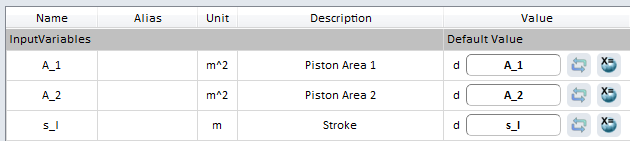
\includegraphics[width=0.8\linewidth]{gfx/advancedusage/systemparameters.png}

It is also possible to choose parameters from a list, by clicking on the globe item to the right of the parameter value. Now do the same thing for the other cylinder. Both cylinders will now use the area and stroke parameters defined in the system parameters widget. If you like to, you can try a few simulations and see that it works as expected.
\end{enumerate}

\section{Subsystems}
Large model diagrams can be made simpler and less confusing by moving groups of components to \textit{subsystems}. A subsystem is practically a component consisting of a system of other components. We will now make a subsystems of the two postion servos.

\begin{enumerate}
\item \textbf{Add a subsystem component} \\
Locate the \textit{Subsystem} component in the library with the same name and add it to the model:
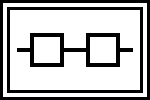
\includegraphics{gfx/advancedusage/subsystem.pdf}

\item\textbf{Select and cut components}
Select the valve, piston, mass and tank component from the first position servo. Press Ctrl-X to cut the components.

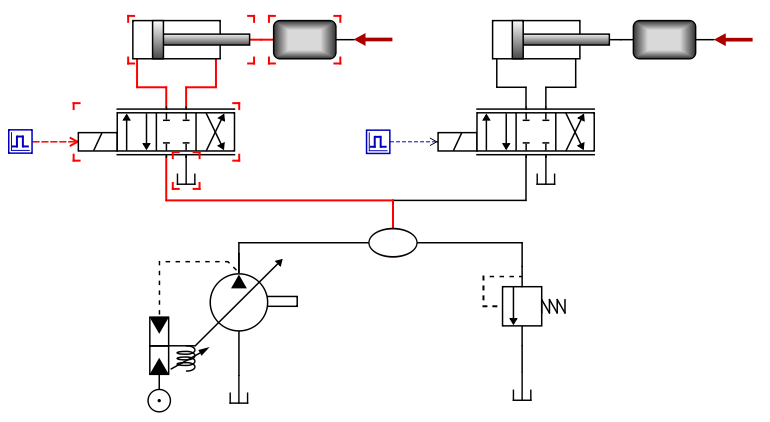
\includegraphics[width=0.8\linewidth]{gfx/advancedusage/componentsforsubsystem.png}

\item\textbf{Enter the subsystem and paste components}
Double-click on the subsystem component to enter the system. Paste the cutted components by pressing Ctrl-V.

\item\textbf{Add container ports}
Ports in subsystems are defined by \textit{container port} components, located in the Subsystem library folder. Add three container ports to the subsystem, and connect them to the three unconnected ports:

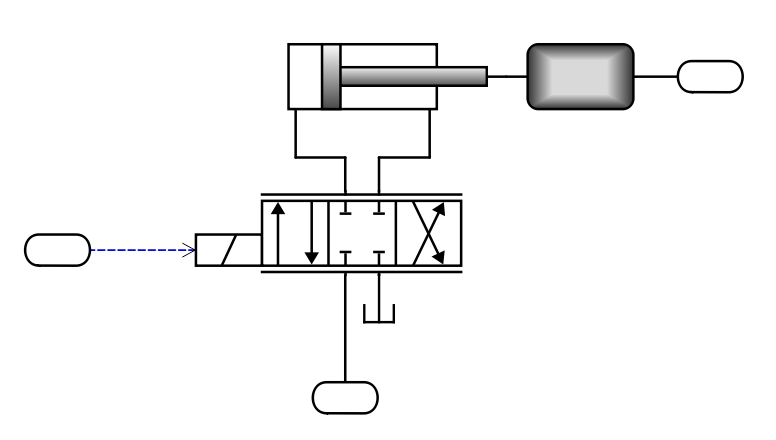
\includegraphics[width=0.6\linewidth]{gfx/advancedusage/systemports.png}

\item\textbf{Connect the subsystem to the model}
Return to the top-level system by clicking on the button at the top left corner of the model. The subsystem now has three ports, representing the container ports. Connect them to the model as shown below:

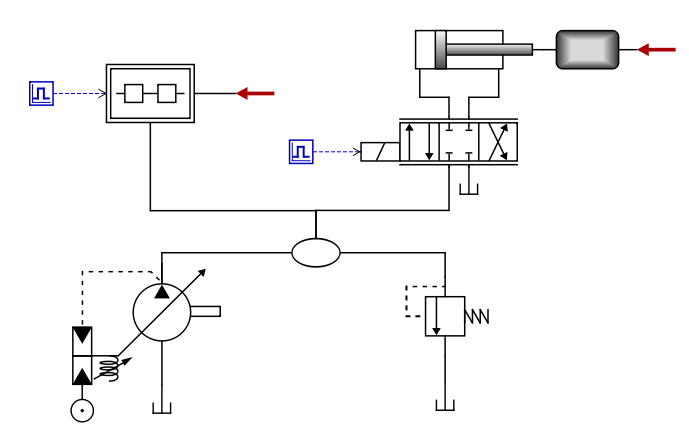
\includegraphics[width=0.8\linewidth]{gfx/advancedusage/connectedsubsystem.png}

\item\textbf{Add parameters to subsystem}
Subsystems can have parameters, just like other components. These are created by adding system parameters to the subsystem. Enter the subsystem by double-clicking on it and add the same three system parameters as we added in the previous section (A\_1, A\_2 and s\_l). Then leave the subsystem and return to the top-level system again. Now right-click on the subsystem component and click on \textit{Properties} in the drop-down menu. Go to the \textit{System Parameters} tab. Here we can change the value of the subsystem parameters, which in turn will affect the piston component. System parameters in the top-level system can be propagated down to the subsystem by setting the value of each system parameter to the name of the top-level system parameter, as in the figure below:

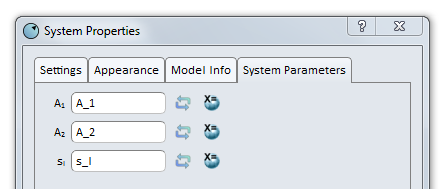
\includegraphics[width=0.6\linewidth]{gfx/advancedusage/subsystemparameters.png}

Everything will now work exactly as before we added the subsystem. If you want to, you can redo the process and create a subsystem for the second postion servo as well.

\end{enumerate}

- Gör ett subsystem av respektive servo
- Låt systemparameten propagera nedåt

\section{Scripting}
- Beskriv hjälpkommandot
- Visa hur man kan ändra parametrar (med och utan wildcard)
- Visa hur man kan plotta data
- Visa hur man kan simulera
- Visa pwd-kommandot
- Gör en skriptfil som simlerar 5 gånger med olika parametrar och plottar resultatet

\begin{lstlisting}[basicstyle=\ttfamily]
rmvar Position_Sensor.out.y@*
GainP.k.y=0.02
i=0
while(i<5)
  sim
  GainP.k.y = GainP.k.y+0.005
  i=i+1
repeat
chpv Position_Sensor.out.y@*
\end{lstlisting}

\section{Importing Data}
- Importera en körcykel för en av cylindrarna från en CSV-fil
- Importera även filen som variabel

\section{Exporting Data}
- Beskriv hur man exporterar från plottfönstret
- Beskriv hur man exporterar från HCOM

\end{document}